
%% bare_conf.tex
%% V1.3
%% 2007/01/11
%% by Michael Shell
%% See:
%% http://www.michaelshell.org/
%% for current contact information.
%%
%% This is a skeleton file demonstrating the use of IEEEtran.cls
%% (requires IEEEtran.cls version 1.7 or later) with an IEEE conference paper.
%%
%% Support sites:
%% http://www.michaelshell.org/tex/ieeetran/
%% http://www.ctan.org/tex-archive/macros/latex/contrib/IEEEtran/
%% and
%% http://www.ieee.org/

%%*************************************************************************
%% Legal Notice:
%% This code is offered as-is without any warranty either expressed or
%% implied; without even the implied warranty of MERCHANTABILITY or
%% FITNESS FOR A PARTICULAR PURPOSE! 
%% User assumes all risk.
%% In no event shall IEEE or any contributor to this code be liable for
%% any damages or losses, including, but not limited to, incidental,
%% consequential, or any other damages, resulting from the use or misuse
%% of any information contained here.
%%
%% All comments are the opinions of their respective authors and are not
%% necessarily endorsed by the IEEE.
%%
%% This work is distributed under the LaTeX Project Public License (LPPL)
%% ( http://www.latex-project.org/ ) version 1.3, and may be freely used,
%% distributed and modified. A copy of the LPPL, version 1.3, is included
%% in the base LaTeX documentation of all distributions of LaTeX released
%% 2003/12/01 or later.
%% Retain all contribution notices and credits.
%% ** Modified files should be clearly indicated as such, including  **
%% ** renaming them and changing author support contact information. **
%%
%% File list of work: IEEEtran.cls, IEEEtran_HOWTO.pdf, bare_adv.tex,
%%                    bare_conf.tex, bare_jrnl.tex, bare_jrnl_compsoc.tex
%%*************************************************************************

% *** Authors should verify (and, if needed, correct) their LaTeX system  ***
% *** with the testflow diagnostic prior to trusting their LaTeX platform ***
% *** with production work. IEEE's font choices can trigger bugs that do  ***
% *** not appear when using other class files.                            ***
% The testflow support page is at:
% http://www.michaelshell.org/tex/testflow/



% Note that the a4paper option is mainly intended so that authors in
% countries using A4 can easily print to A4 and see how their papers will
% look in print - the typesetting of the document will not typically be
% affected with changes in paper size (but the bottom and side margins will).
% Use the testflow package mentioned above to verify correct handling of
% both paper sizes by the user's LaTeX system.
%
% Also note that the "draftcls" or "draftclsnofoot", not "draft", option
% should be used if it is desired that the figures are to be displayed in
% draft mode.
%
\documentclass[10pt, conference, compsocconf]{ieee}
\usepackage[lined, boxed]{algorithm2e}
\usepackage{times}
\usepackage{subfigure}
\usepackage{epsfig}
\usepackage{multirow}
\usepackage{listings}
\usepackage{url}
\usepackage{amsfonts}
\usepackage{amsmath}
\usepackage{framed}

% Add the compsocconf option for Computer Society conferences.
%
% If IEEEtran.cls has not been installed into the LaTeX system files,
% manually specify the path to it like:
% \documentclass[conference]{../sty/IEEEtran}





% Some very useful LaTeX packages include:
% (uncomment the ones you want to load)


% *** MISC UTILITY PACKAGES ***
%
%\usepackage{ifpdf}
% Heiko Oberdiek's ifpdf.sty is very useful if you need conditional
% compilation based on whether the output is pdf or dvi.
% usage:
% \ifpdf
%   % pdf code
% \else
%   % dvi code
% \fi
% The latest version of ifpdf.sty can be obtained from:
% http://www.ctan.org/tex-archive/macros/latex/contrib/oberdiek/
% Also, note that IEEEtran.cls V1.7 and later provides a builtin
% \ifCLASSINFOpdf conditional that works the same way.
% When switching from latex to pdflatex and vice-versa, the compiler may
% have to be run twice to clear warning/error messages.






% *** CITATION PACKAGES ***
%
%\usepackage{cite}
% cite.sty was written by Donald Arseneau
% V1.6 and later of IEEEtran pre-defines the format of the cite.sty package
% \cite{} output to follow that of IEEE. Loading the cite package will
% result in citation numbers being automatically sorted and properly
% "compressed/ranged". e.g., [1], [9], [2], [7], [5], [6] without using
% cite.sty will become [1], [2], [5]--[7], [9] using cite.sty. cite.sty's
% \cite will automatically add leading space, if needed. Use cite.sty's
% noadjust option (cite.sty V3.8 and later) if you want to turn this off.
% cite.sty is already installed on most LaTeX systems. Be sure and use
% version 4.0 (2003-05-27) and later if using hyperref.sty. cite.sty does
% not currently provide for hyperlinked citations.
% The latest version can be obtained at:
% http://www.ctan.org/tex-archive/macros/latex/contrib/cite/
% The documentation is contained in the cite.sty file itself.






% *** GRAPHICS RELATED PACKAGES ***
%
\ifCLASSINFOpdf
  % \usepackage[pdftex]{graphicx}
  % declare the path(s) where your graphic files are
  % \graphicspath{{../pdf/}{../jpeg/}}
  % and their extensions so you won't have to specify these with
  % every instance of \includegraphics
  % \DeclareGraphicsExtensions{.pdf,.jpeg,.png}
\else
  % or other class option (dvipsone, dvipdf, if not using dvips). graphicx
  % will default to the driver specified in the system graphics.cfg if no
  % driver is specified.
  % \usepackage[dvips]{graphicx}
  % declare the path(s) where your graphic files are
  % \graphicspath{{../eps/}}
  % and their extensions so you won't have to specify these with
  % every instance of \includegraphics
  % \DeclareGraphicsExtensions{.eps}
\fi
% graphicx was written by David Carlisle and Sebastian Rahtz. It is
% required if you want graphics, photos, etc. graphicx.sty is already
% installed on most LaTeX systems. The latest version and documentation can
% be obtained at: 
% http://www.ctan.org/tex-archive/macros/latex/required/graphics/
% Another good source of documentation is "Using Imported Graphics in
% LaTeX2e" by Keith Reckdahl which can be found as epslatex.ps or
% epslatex.pdf at: http://www.ctan.org/tex-archive/info/
%
% latex, and pdflatex in dvi mode, support graphics in encapsulated
% postscript (.eps) format. pdflatex in pdf mode supports graphics
% in .pdf, .jpeg, .png and .mps (metapost) formats. Users should ensure
% that all non-photo figures use a vector format (.eps, .pdf, .mps) and
% not a bitmapped formats (.jpeg, .png). IEEE frowns on bitmapped formats
% which can result in "jaggedy"/blurry rendering of lines and letters as
% well as large increases in file sizes.
%
% You can find documentation about the pdfTeX application at:
% http://www.tug.org/applications/pdftex





% *** MATH PACKAGES ***
%
%\usepackage[cmex10]{amsmath}
% A popular package from the American Mathematical Society that provides
% many useful and powerful commands for dealing with mathematics. If using
% it, be sure to load this package with the cmex10 option to ensure that
% only type 1 fonts will utilized at all point sizes. Without this option,
% it is possible that some math symbols, particularly those within
% footnotes, will be rendered in bitmap form which will result in a
% document that can not be IEEE Xplore compliant!
%
% Also, note that the amsmath package sets \interdisplaylinepenalty to 10000
% thus preventing page breaks from occurring within multiline equations. Use:
%\interdisplaylinepenalty=2500
% after loading amsmath to restore such page breaks as IEEEtran.cls normally
% does. amsmath.sty is already installed on most LaTeX systems. The latest
% version and documentation can be obtained at:
% http://www.ctan.org/tex-archive/macros/latex/required/amslatex/math/





% *** SPECIALIZED LIST PACKAGES ***
%
%\usepackage{algorithmic}
% algorithmic.sty was written by Peter Williams and Rogerio Brito.
% This package provides an algorithmic environment fo describing algorithms.
% You can use the algorithmic environment in-text or within a figure
% environment to provide for a floating algorithm. Do NOT use the algorithm
% floating environment provided by algorithm.sty (by the same authors) or
% algorithm2e.sty (by Christophe Fiorio) as IEEE does not use dedicated
% algorithm float types and packages that provide these will not provide
% correct IEEE style captions. The latest version and documentation of
% algorithmic.sty can be obtained at:
% http://www.ctan.org/tex-archive/macros/latex/contrib/algorithms/
% There is also a support site at:
% http://algorithms.berlios.de/index.html
% Also of interest may be the (relatively newer and more customizable)
% algorithmicx.sty package by Szasz Janos:
% http://www.ctan.org/tex-archive/macros/latex/contrib/algorithmicx/




% *** ALIGNMENT PACKAGES ***
%
%\usepackage{array}
% Frank Mittelbach's and David Carlisle's array.sty patches and improves
% the standard LaTeX2e array and tabular environments to provide better
% appearance and additional user controls. As the default LaTeX2e table
% generation code is lacking to the point of almost being broken with
% respect to the quality of the end results, all users are strongly
% advised to use an enhanced (at the very least that provided by array.sty)
% set of table tools. array.sty is already installed on most systems. The
% latest version and documentation can be obtained at:
% http://www.ctan.org/tex-archive/macros/latex/required/tools/


%\usepackage{mdwmath}
%\usepackage{mdwtab}
% Also highly recommended is Mark Wooding's extremely powerful MDW tools,
% especially mdwmath.sty and mdwtab.sty which are used to format equations
% and tables, respectively. The MDWtools set is already installed on most
% LaTeX systems. The lastest version and documentation is available at:
% http://www.ctan.org/tex-archive/macros/latex/contrib/mdwtools/


% IEEEtran contains the IEEEeqnarray family of commands that can be used to
% generate multiline equations as well as matrices, tables, etc., of high
% quality.


%\usepackage{eqparbox}
% Also of notable interest is Scott Pakin's eqparbox package for creating
% (automatically sized) equal width boxes - aka "natural width parboxes".
% Available at:
% http://www.ctan.org/tex-archive/macros/latex/contrib/eqparbox/





% *** SUBFIGURE PACKAGES ***
%\usepackage[tight,footnotesize]{subfigure}
% subfigure.sty was written by Steven Douglas Cochran. This package makes it
% easy to put subfigures in your figures. e.g., "Figure 1a and 1b". For IEEE
% work, it is a good idea to load it with the tight package option to reduce
% the amount of white space around the subfigures. subfigure.sty is already
% installed on most LaTeX systems. The latest version and documentation can
% be obtained at:
% http://www.ctan.org/tex-archive/obsolete/macros/latex/contrib/subfigure/
% subfigure.sty has been superceeded by subfig.sty.



%\usepackage[caption=false]{caption}
%\usepackage[font=footnotesize]{subfig}
% subfig.sty, also written by Steven Douglas Cochran, is the modern
% replacement for subfigure.sty. However, subfig.sty requires and
% automatically loads Axel Sommerfeldt's caption.sty which will override
% IEEEtran.cls handling of captions and this will result in nonIEEE style
% figure/table captions. To prevent this problem, be sure and preload
% caption.sty with its "caption=false" package option. This is will preserve
% IEEEtran.cls handing of captions. Version 1.3 (2005/06/28) and later 
% (recommended due to many improvements over 1.2) of subfig.sty supports
% the caption=false option directly:
%\usepackage[caption=false,font=footnotesize]{subfig}
%
% The latest version and documentation can be obtained at:
% http://www.ctan.org/tex-archive/macros/latex/contrib/subfig/
% The latest version and documentation of caption.sty can be obtained at:
% http://www.ctan.org/tex-archive/macros/latex/contrib/caption/




% *** FLOAT PACKAGES ***
%
%\usepackage{fixltx2e}
% fixltx2e, the successor to the earlier fix2col.sty, was written by
% Frank Mittelbach and David Carlisle. This package corrects a few problems
% in the LaTeX2e kernel, the most notable of which is that in current
% LaTeX2e releases, the ordering of single and double column floats is not
% guaranteed to be preserved. Thus, an unpatched LaTeX2e can allow a
% single column figure to be placed prior to an earlier double column
% figure. The latest version and documentation can be found at:
% http://www.ctan.org/tex-archive/macros/latex/base/



%\usepackage{stfloats}
% stfloats.sty was written by Sigitas Tolusis. This package gives LaTeX2e
% the ability to do double column floats at the bottom of the page as well
% as the top. (e.g., "\begin{figure*}[!b]" is not normally possible in
% LaTeX2e). It also provides a command:
%\fnbelowfloat
% to enable the placement of footnotes below bottom floats (the standard
% LaTeX2e kernel puts them above bottom floats). This is an invasive package
% which rewrites many portions of the LaTeX2e float routines. It may not work
% with other packages that modify the LaTeX2e float routines. The latest
% version and documentation can be obtained at:
% http://www.ctan.org/tex-archive/macros/latex/contrib/sttools/
% Documentation is contained in the stfloats.sty comments as well as in the
% presfull.pdf file. Do not use the stfloats baselinefloat ability as IEEE
% does not allow \baselineskip to stretch. Authors submitting work to the
% IEEE should note that IEEE rarely uses double column equations and
% that authors should try to avoid such use. Do not be tempted to use the
% cuted.sty or midfloat.sty packages (also by Sigitas Tolusis) as IEEE does
% not format its papers in such ways.





% *** PDF, URL AND HYPERLINK PACKAGES ***
%
%\usepackage{url}
% url.sty was written by Donald Arseneau. It provides better support for
% handling and breaking URLs. url.sty is already installed on most LaTeX
% systems. The latest version can be obtained at:
% http://www.ctan.org/tex-archive/macros/latex/contrib/misc/
% Read the url.sty source comments for usage information. Basically,
% \url{my_url_here}.





% *** Do not adjust lengths that control margins, column widths, etc. ***
% *** Do not use packages that alter fonts (such as pslatex).         ***
% There should be no need to do such things with IEEEtran.cls V1.6 and later.
% (Unless specifically asked to do so by the journal or conference you plan
% to submit to, of course. )


% correct bad hyphenation here
%\hyphenation{op-tical net-works semi-conduc-tor}


\begin{document}
%
% paper title
% can use linebreaks \\ within to get better formatting as desired
\title{How to Group Crashes Effectively: Comparing Manually and Automatically Grouped Crash Dumps}


% author names and affiliations
% use a multiple column layout for up to two different
% affiliations

\author{\IEEEauthorblockN{Wei Le and Daniel Krutz}
\IEEEauthorblockA{Rochester Institute of Technology\\One Lomb Memorial Drive, Rochester NY 14623\\ \{wei.le,dxkvse\}@rit.edu}
}

% conference papers do not typically use \thanks and this command
% is locked out in conference mode. If really needed, such as for
% the acknowledgment of grants, issue a \IEEEoverridecommandlockouts
% after \documentclass

% for over three affiliations, or if they all won't fit within the width
% of the page, use this alternative format:
% 
%\author{\IEEEauthorblockN{Michael Shell\IEEEauthorrefmark{1},
%Homer Simpson\IEEEauthorrefmark{2},
%James Kirk\IEEEauthorrefmark{3}, 
%Montgomery Scott\IEEEauthorrefmark{3} and
%Eldon Tyrell\IEEEauthorrefmark{4}}
%\IEEEauthorblockA{\IEEEauthorrefmark{1}School of Electrical and Computer Engineering\\
%Georgia Institute of Technology,
%Atlanta, Georgia 30332--0250\\ Email: see http://www.michaelshell.org/contact.html}
%\IEEEauthorblockA{\IEEEauthorrefmark{2}Twentieth Century Fox, Springfield, USA\\
%Email: homer@thesimpsons.com}
%\IEEEauthorblockA{\IEEEauthorrefmark{3}Starfleet Academy, San Francisco, California 96678-2391\\
%Telephone: (800) 555--1212, Fax: (888) 555--1212}
%\IEEEauthorblockA{\IEEEauthorrefmark{4}Tyrell Inc., 123 Replicant Street, Los Angeles, California 90210--4321}}




% use for special paper notices
%\IEEEspecialpapernotice{(Invited Paper)}




% make the title area
\maketitle

Mobile applications~(\emph{apps}) are ubiquitous in today's world, allowing us to do everything from update our Facebook profile to trading of stocks at the push of a button. Unfortunately, with this great power also comes extreme dangers. User's may unknowingly download a malicious application, while developer's may create an app with security vulnerabilities which may lead to a range of security threats ranging from data theft to device locking. Recent studies have shown that 68-77\% of Android apps are susceptible to just a single SSL vulnerability.
This article present an easy to use, publicly available website and data set located to assist developers, researchers, users and educators/students with better understanding Android app security. The underlying infrastructure contains a number of security and static analysis tools which are automatically run over one thousands open source Android apps from the F-Droid repository. The Androsec portal represents the apps source code, the security scores, and analyzed results from various tools and provides several features for the users to query this analytical dataset.

%Mobile applications~(\emph{apps}) are ubiquitous in today's world, allowing us to do everything from update our Facebook profile to trading of stocks at the push of a button. Unfortunately, with this great power also comes extreme dangers. User's may unknowingly download a malicious application, while developer's may create an app with security vulnerabilities which may lead to a range of security threats ranging from data theft to device locking{\todo{check}}. Recent studies have shown that 68-77\% of Android apps are susceptible to just a single SSL vulnerability.

%Developers must not only be aware of both how to create secure apps, but of the importance of developing secure apps as well. Conversely, user's should have quality, easily accessible information to enable them to make an informed, objective decision about which apps and app versions off the best level of security. Researchers pave the way for new discoveries in both the process of developing secure software, and in understanding why vulnerabilities take place at a technical level. In order to carry out both qualitative and quantitative studies, researchers need quality and accessible data sets in which to analyze. Students need quality data, examples and exercises to educate them about the importance and process of creating secure apps.

%We have created an easy to use, publicly available website an data set located at~\url{http://androsec.rit.edu} to assist developers, researchers, users and educators/students with better understanding Android app security,. We created this by first downloading 1,179 open source Android apps from the F-Droid repository, which we then analyzed using several security and quality static analysis tools. The site contains both comprehensive and easy to use reports, along with several in-depth data sets for researchers to download. \dan{Should this be shortened?}



%This instruction


%User's should be educated


%Developers need to protect
%User's need to be educated
%Researchers

%Briefly describe our site/process

\begin{IEEEkeywords}
Crash Dumps, Call Stacks, Grouping, Similarity
\end{IEEEkeywords}


%Agile Architecture, no upfront design

%Design thinking integrated into coding

%Advocates design thinking while programming

%No documentation of architecture

%Design Knowledge is tacit in the head of people

%Use social ways to maintain knowledge



%% Introduction to Agile development methodologies

Agile software development is a method of managing software projects to make them more adaptable to change and to reduce costs associated with unnecessary documentation. Agile development emphasizes close collaboration between developers and business experts, frequent face to face communication, continual delivery of incremental working software, and self organizing teams. This is a stark contrast to development techniques such as Waterfall, that typically require significant amounts of up front requirements analysis, architecture design and continuous documentation. This often makes project changes more difficult and expensive.

The reduction of excessive up front design and unneeded formal architectural documentation increases the necessity for other methods of addressing quality, communication, and interactions between developers and stakeholders. In agile software development, architecture design is integrated with coding activities, advocating less up front design and more incremental architectural spikes to address each quality requirements. In such an environment, there is also less emphasize on documenting architectural knowledge from driving requirements to the adopted patterns, tactics and styles. The rationale behind these choices are maintained socially through practices such as pair programming, collective ownership and stand up meetings.

Currently, agile techniques are supported with tools which promote core agile practices. For example there are several mature tools for code refactoring and test driven design~\cite{Alves:2014:RRA:2635868.2661674, Moghadam:2011:CTA:1984732.1984742, Nongpong:2012:ICS:2519037}. Unfortunately, there are few tools which assist developers in agile architecture development, design maintenance~\cite{ICSE2012,Erosion} and documentation. Architecture centric tools~\cite{KA,AntonyTool,DBLP:conf/qosa/LeeK08} assume that an up front architecture design processes exist and heavy design artifacts are created. This makes them impractical in many iterative incremental projects with small cycles of design and often leads developers to not adopt these tools. Instead, they are often forced to rely upon social techniques to develop, communicate, and maintain their architecture.

The lack of architecture centric tools that fit the agile development paradigm and culture can increase the chances of quality degradation, where the implementation of architectural choices to satisfy quality concerns are drifted from the initial intends resulting design erosion and degradation of software qualities. In Robert Martin's recent book entitled ``Agile Software Development - Principles, Patterns, and Practices''~\cite{Martin2002}, he commented that while developers may initially release a system that meets the intended design, it does not take long before ``the software starts to rot like a piece of bad meat'' leading  to problems such as rigidity, fragility, and unnecessary complexity of the design. 

This problem is exacerbated by the fact that popular software engineering tools and environments fail to make underlying design decisions visible to programmers. This results in maintainers not being kept fully informed of the relevant underlying patterns, tactics, and constraints as they build, maintain, and refactor a software system~\cite{Booch:DrawPicture}.

In this paper, we introduce a pluggable tool~\emph{Archie}, which can be used to support different agile-architecture development activities. This tool was initially developed to support integrated architecture development and maintenance. However the automation features of Archie makes it suitable for agile projects. Archie has features for helping developers devise incremental architectural choices, proactively sharing design knowledge with programmers, and keeping them informed of underlying architectural decisions during coding activities. Archie helps developers to perform change impact analysis of architectural concerns at the code level, and provides infrastructure to enable the concept of ``Design Ownership'', supporting the developers to obtain accountability for their design choices.


\section{Dataset and Methodologies}~\label{sec:approach}

In this section, we present how our dataset is constructed and how the information regarding a-groups and m-groups is collected for comparison.

\subsection{Dataset: a-groups and m-groups}
Our study subject is {\it crash dumps}.  When a crash occurs at the client side, a crash dump is generated by the deployed crash management system. Typically, it captures the program state at the crash as well as static information about the system and software. For example, a crash dump returned by Mozilla Crash Reporter mainly include: 1) call stacks of each active thread at the crash, 2) exception types captured at the crash such as EXCEPTION\_ACCESS\_VIOLATION\_WRITE, and 3) operating system, software and their versions, as well as the building, installation and crashing dates and time.  When a user clicks the {\it submit crash report} button, the crash dumps are sent back to the server for postmortem analysis.  Mozilla Crash Reporter system organizes groups of crash dumps based on applications. For each application, it ranks most frequently occurred crash dump groups within a certain time window. 

A user can also send in crash information manually through Bugzilla~\cite{bugzilla}, in which case, the crash information is constructed in ad-hoc based on the users' judgment. Compared to crash dumps generated automatically, the report in Bugzilla may contain additional information, such as 1) reproduce steps that lead to crashes, 2) piece of code that is suspected to cause the crash, 3) the URL visited when the application crashes, 4) expected results, 5) the other bugs that may be relevant, and 6) any connections to groups of crash dumps reported by Mozilla Crash Reporter. 

In Figure~\ref{fig:dataprocess}, we show how a-groups and m-groups in our study are constructed. The groups of crash dumps are selected from both Mozilla Crash Reporter and Bugzilla, dated between 2/16-4/16/2012, across five applications including {\it Firefox}, {\it Thunderbird}, {\it Fennec}, {\it FennecAndroid} and {\it SeaMonkey}. For a-groups, we collect maximally 300 top crash dump groups for each application. 


For m-groups, we inspect the summary page Mozilla presents for each a-group, shown in Figure~\ref{fig:bugzilla}. From the page, we find Bugzilla entries that are correlated to the a-group, shown in Figure~\ref{fig:bugzilla}. We recursively search each correlated Bugzilla entry to find more Bugzilla entries that are confirmed to be relevant. The crash dumps reported in these Bugzilla entries constitute an m-group. As an example, in Figure~\ref{fig:dataprocess}, $b_1$ and $b_2$ are the two Bugzilla entries found relevant to {\it a-group} and $b_3$ is identified by recursively inspecting $b_1$ and $b_2$ for related bugs. The Bugzilla entries also contain the developers' discussions on how to diagnose the crash dumps. 

\begin{figure}[!htb]
\centering
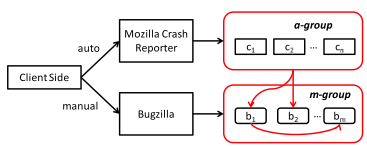
\includegraphics[width = 8.4cm, angle = 0]{approach1.ps}
\caption{\small Collect a-Groups and m-Groups~\label{fig:dataprocess}}
\normalsize
\end{figure}

\begin{figure}[!htb]
\centering
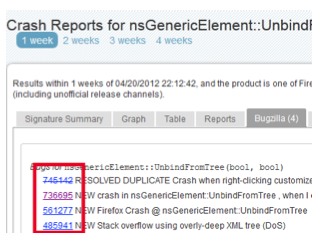
\includegraphics[width = 5.4cm, angle = 0]{bugzilla.ps}
\caption{Link a-group and m-group~\label{fig:bugzilla}}
\normalsize
\end{figure}

Table~\ref{tab:dataset} summarizes the dataset we collected. Under {\it T$_g$}, we display the number of a-groups and m-groups studied for each application. The first four applications contain more than 300 a-groups and by setting a threshold 300, we successfully collected 297 to 299 a-groups. For each application, we randomly select 20 a-groups, based on which we construct m-groups, as explained in Figure~\ref{fig:dataprocess}. Under {\it T$_b$}, we count the total number of Bugzilla entries associated with the 20 m-groups. In each Bugzilla entry, users can report multiple crash dumps related to the bug. Under {\it T$_c$}, we list the total number of crash dumps in the m-groups. The data indicate that on average, each Bugzilla entries contain 2--3 crash dumps.

\begin{table}
\caption{Dataset from 5 Mozilla Applications\label{tab:dataset}}
\resizebox{\columnwidth}{!}{
\begin{tabular}{|l||c|c||c|c|c|}\hline

\multirow{2}{*}{Program} & \multicolumn{2}{|c||}{a-Groups} & \multicolumn{3}{|c|}{m-Groups} \\\cline{2-6}

&T$_g$&T$_c$&T$_g$&T$_b$&T$_c$ \\ \hline\hline

Firefox 14.0a1&298&18316&20&110&233\\ \hline
Thunderbird 10.0&299&3151&20&106&237\\ \hline
Fennec 2.1.2&299&2567&20&87&155\\ \hline
Fennec Android 13.0a1&297&4925&20&90&189\\ \hline
SeaMonkey 2.7.2&257&514&20&59&144\\ \hline

%Firefox 14.0a1&299&18316&1&16/8645&1743&12&20&110&233&3&39&&61\\ \hline
%Thunderbird 10.0&299&3151&16&16/355&1792&32&20&106&237&3&33&1024&93\\ \hline
%Fennec 2.1.2&299&2567&1&16/2233&1792&2&20&87&155&3&24&1456&46\\ \hline
%Fennec Android 13.0a1&168&4925&1&16/993&1165&2&20&90&189&3&24&1456&82\\ \hline
%SeaMonkey 2.7.2&257&514&1&15/15&196&5&20&59&144&3&16&596&6\\ \hline

\end{tabular}
}
\end{table}

\subsection{Comparison Metrics and Approaches}
Given dataset a-groups and m-groups, our goals are to determine whether manual and automatic approaches apply consistent criteria and information to group crashes, and whether the two approaches correlate same types of call stacks. As shown in Figure~\ref{fig:approach}, we compare the groups based on the four metrics, including: 
\begin{itemize}
\item {\it Grouping criteria}: why do we group crash dumps and how the groups can be used?
\item {\it Grouping information}: what information shall we use, and how shall we use it, for more effectively grouping crash dumps?
\item {\it Imprecision in the groups}: when do we group unrelated crash dumps or when do we fail to find the relevant crash dumps? 
\item {\it Characteristics of call stacks}: what are the patterns in call stacks in a-groups and m-groups? How do the characteristics imply the capabilities of the two approaches?
\end{itemize}


\begin{figure}[!htb]
\centering
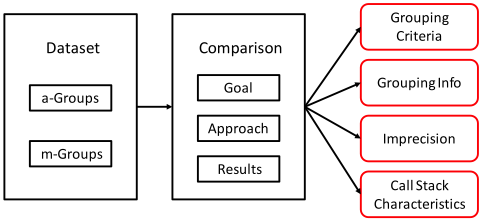
\includegraphics[width = 8.4cm, angle = 0]{approach2.ps}
\caption{Compare a-Groups and m-Groups~\label{fig:approach}}
\normalsize
\end{figure}

To collect information for performing comparisons, we take the following three steps.

{\bf Identifying grouping criteria and information.} For a-groups, we studied documentation related to Mozilla Crash Reporter to understand the criteria and algorithms used. To determine grouping criteria and information used for m-groups, we analyzed  452 Bugzilla entries where the m-groups are determined. For learning grouping criteria, our focus is to determine what relations are established between crash dumps in the group and how developers compare and contrast crash dumps in a group for prioritizing, diagnosing and fixing the code. To obtain information important for correlating crash dumps, we define a set of keywords, representing potential sources of information,  e.g., {\it call stacks}, {\it reproduce steps}, {\it regression windows}, {\it URL}, {\it plugin} and {\it libraries}. Based on these key words, we extract relevant text from the Bugzilla entries. We then count the frequencies at which each type of information is used and also the frequencies at which different types of information are combined in determining a group.

{\bf Determining imprecision in a-groups and m-groups.} In this step, we aim to learn the existence, causes and consequences of imprecision for both of the approaches. To determine imprecision in a-groups, we randomly selected 100 a-groups from our dataset and for each a-group, we analyze the relevant Bugzilla entries that contain diagnostic information for the a-groups. We determine an a-group is imprecise if the developers confirm that the a-group: 1) contains a corrupted signature or call stack, 2) includes crash dumps that should not be correlated, and 3) fails to group crash dumps that should be correlated.  Imprecision in m-groups is caused by developers' mistakes. We inspect developers' discussion logs in the Bugzilla entries and identify cases where developers believe unrelated crash dumps are grouped by mistakes.

{\bf Comparing call stack characteristics.} To compare the capabilities of manual and automatic approaches, we study the patterns in call stacks for a-groups and m-groups. To determine if there is a pattern, we also construct {\it r-groups}; each of the r-groups contains the random number of crash dumps randomly selected from a-groups.  We compare a-groups and m-groups regarding 1) the sizes of groups, including the number of call stacks in each group and the length of the call stacks, and 2) the similarity between call stacks. We compute the metrics in string matching algorithms to measure the similarity between the call stacks, including the {\it Brodie value} ({\it B-Value}), {\it Brodie weight} ({\it B-Weight})~\cite{brodie:automated,brodie:quickly}, longest common substrings ({\it LCS}), and the percentage of identical call stacks in a group ({\it C-Identical}). In the following, we explain how each of the measure is calculated. 

Suppose $m$ is the number of {\it matching lines} between two call stacks, and $l_1$ and $l_2$ are the lengths of the two call stacks. Brodie value $bv$ is computed as:

\[
  bv = \left\{
  \begin{array}{l l}
    m/l_1 & \quad l_1 == l_2\\
    m/((l_1+l_2)/2) & \quad l_1\neq l_2\\
  \end{array} \right.
\]

We consider a {\it matching line} between two call stacks if at location $i$ from the top of the call stacks $C_1$ and $C_2$, the function names $C_1[i]$ and $C_2[i]$ are identical. 

Brodie weight is a string similarity metric improved from the Brodie value. It distinguishes the weight of the functions in call stacks for determining similarity. The assumption is that functions located at the top of the call stack should have more weight than ones located at the bottom. The detailed algorithm of how to compute Brodie weight between two call stacks is given in~\cite{brodie:automated}.

%\IncMargin{1em}
%\LinesNumbered
%\begin{algorithm}[!htb]
%\SetFuncSty{bf}
%\SetKwData{ans}{Unsolved}
%\SetKwFunction{icfg}{BuildICFG}
%\SetKwInOut{Input}{Input}
%\SetKwInOut{Output}{Output}

%\Input{Specification of Fault, $spec$}
%\Output{Calls to {\bf MatchFSignature}, {\bf MatchDSignature};\\

%A repository of function definitions, $R$}
%\BlankLine
 	  
%\caption{Generating Analysis\label{alg:generation}} %{\bf MatchFSignature} and {\bf MatchDSignature}
%\normalsize
%\end{algorithm}

We obtain the Brodie value/weight for a group by adding up the Brodie value/weight for every two call stacks in the group and then dividing the times of comparisons. Finally, we get an average across groups for an application.

To compute LCS across all the call stacks in a group, we first detect a set of common substrings between two call stacks. We then determine whether other call stacks in the group contain the same common substrings. The comparison is performed between the average LCS across a-groups and the average LCS across m-groups for an application. 

The {\it C-Identical} identifies the maximum number of crash dumps in a group that are actually identical, calculated by $n_i$/$n$. In an a-group or m-group, we may find several subgroups, within which, crash dumps are identical. $n_i$ here is the number of identical call stacks in the largest subgroup and $n$ is the size of the a-group or m-group.
\section{Results}~\label{sec:results}
In this section, we present our comparison results and our insights for designing better grouping tools.

\subsection{Comparison based on Grouping Criteria}
RQ1: Why do we group crash dumps?
\begin{enumerate}
\item Besides grouped based on the same root cause, crash dumps can also be correlated if the patch to one crash is the cause for another crash.
\item Developers also group crash dumps if they can be conveniently fixed together, for example, by a same developer.
\item Diagnosing a group of crash dumps can be beneficial: first, a group of symptoms help determine general manifestation of a bug; second, a group of similar call stacks potentially enable automatic bug localizations. 
\end{enumerate}

\begin{table}[!htb]
\centering
\caption{Grouping Criteria for m-Groups\label{tab:goal}}
\resizebox{\columnwidth}{!}{
\begin{tabular}{|l||l|l|}\hline
Grouping Criteria&Goals\\\hline\hline
\multirow{4}{*}{Same Root Cause}&Fix one to fix all in the group\\\cline{2-2}
&Determine if a given new crash is fixed\\\cline{2-2}
&Localize bugs via comparing similar stacks\\\cline{2-2}
&Learn bug manifestation to prioritize them\\\hline\hline
\multirow{2}{*}{Related Root Cause}&Localize root causes if fix to previous\\
&crashes is the cause for the current crash\\\hline\hline
\multirow{2}{*}{Who Fix the Bug}&Find experts who can fix a group of bugs\\
&from the same code region or of same types\\\hline
\end{tabular}
}
\end{table}

%\begin{figure}
%\begin{minipage}[b]{\textwidth}
%\centering
%\includegraphics[width = \columnwidth, angle = 0]{group.ps}
%\end{minipage}
%\caption{Fault Localization Based On Call Stacks~\label{fig:group}}
%\end{figure}

For automatic approaches that compare call stack similarity for grouping crash dumps, the implied grouping criterion is that the crash dumps in a group should share the root cause. However, we find that the grouping criteria applied in manual diagnosis are more diverse and flexible. 

In Table~\ref{tab:goal}, we summarize our discoveries. Similar to automatic approaches, in many cases, developers correlate crash dumps if they believe these crashes are originated from the same bug in the code. In another word, if we introduce a fix based on any crash in the group, we can fix all the crash dumps grouped, and if a new crash dump is determined to belong to the group, we do not need to further diagnose it.

Interestingly, although the goal of grouping crash dumps is to avoid repeatedly diagnosing crash dumps caused by the same root cause, developers sometimes still compare multiple crash dumps in the same group for determining the types and locations of a bug. It indicates that a group of crash dumps can be more informative than individual crash dumps in helping diagnose failures. For example, a same bug may cause completely different symptoms, and we find a case where developers prioritize a group of crash dumps because one of the crashes have the serve symptom related to a security attack. 

As shown in the table, developers also correlate crash dumps if the root causes that lead to the crashes have a temporal or locality relationship. In our study, we find cases where one crash is caused by an incomplete/incorrect fix to the other crashes. Developers believe that correlating these crashes can help quickly identify the cause and the fix for the newly generated crashes.

In addition, developers group crash dumps using the criterion of who can fix them. Here, the components where the crashes occur, together with the bug types, are used to determine the groups. The goal is to better distribute the debugging tasks to people who are most familiar with the code and the bug types.

\subsection{Comparison based on Grouping Information}

RQ2: What information shall we use to group crashes?
\begin{enumerate}
\item Call stacks, build information and reproduce steps are the three main sources for developers to group crashes.
\item Developers frequently correlate multiple sources of information for determining the groups. For example, developers once linked call stacks and reproduce steps by comparing call stacks in crash dumps with the call stack in a non-crash thread.
\item Developers correlate crash dumps across applications to determine if the root cause is located in the shared libraries or plugins.
\item Different versions of programs can contain the same piece of problematic code, and thus we should enable the grouping across different versions of the code.
\end{enumerate}


\begin{figure*}
%\begin{minipage}[b]{\textwidth}
%\subfigure[Same Signature, Different Causes]{
\subfigure[List of Information Source]{
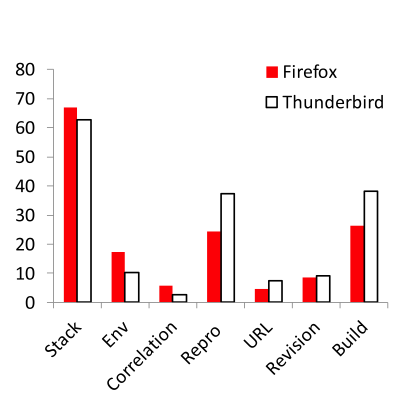
\includegraphics[width = 6.6 cm, angle = 0]{Info1.ps}
~\label{fig:ind}
}
\subfigure[Linking Multiple Sources]{
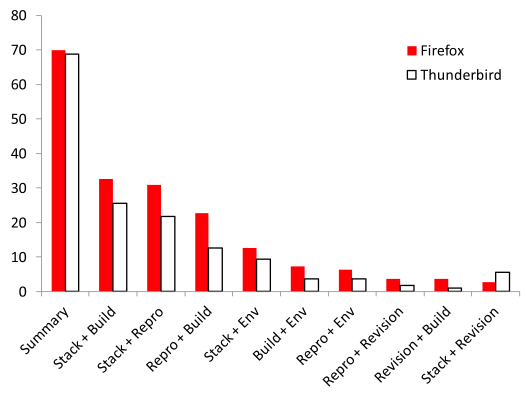
\includegraphics[width = 9.0 cm, angle = 0]{Info2.ps}
~\label{fig:multi}
}
%\end{minipage}
\caption{Information Used for Manually Grouping Crash Dumps~\label{fig:stack}}
\end{figure*}

Mozilla Crash Reporter automatically groups crash dumps by matching 1) the version of software where the crash dumps are originated; and 2) the function call on the top of the call stack at the crash, called {\it signature}. On the contrarily, developers use a variety of information. No systematic way is applied to choose which source of information should be used for determining a particular group of crash dumps.

We studied a total of 40 m-groups from Firefox and Thunderbird. We find that developers generally apply three types of information for grouping crash dumps: 1) white-box information, i.e., crash symptoms related to code including call stacks and their signatures, 2) black-box testing information, e.g. steps on triggering the bug, and 3) information related to software versions, such as build time and revision histories. 

We summarize our analysis results in Figure~\ref{fig:stack}. On the left, we rank a list of information source developers frequently use in determining crash dump groups, and on the right we show the correlation of these sources applied in manual diagnosis. The $y$-axis presents the percentage of crash dumps that are grouped using the specific source(s) of information.

In Figure~\ref{fig:ind}, along the $x$-axis, {\it Stack} represents call stacks. {\it Env} indicates the plugins and libraries involved in the crash. {\it Correlation}, used by Mozilla Crash Reporter, specifies how often a signature and a .dll component are simultaneously witnessed in a crash. For example, given a set of call stacks, we count that a certain signature occurs 10 times, and among the 5 times, a specific .dll also occurs; in this case, the correlation ratio between the signature and the component is 50\%. {\it Repro} and {\it URL} indicate two relevant types of testing information. {\it Repro} represents the steps taken to reproduce the bug and {\it URL} refers to a list of URL visited before an application crashes. {\it Revision} is a list of changes made to the application shortly before a crash. Finally, {\it Build} gives the date and time to indicate when the application is built and installed, as well as the version of operating system where the application runs.

Figure~\ref{fig:ind} shows that call stack, build information and reproduce steps are the three most frequently used sources. For Firefox, 67\% of the crash dumps were grouped using call stacks, 26.4\% applied build information and 24.5\% were determined using reproduce steps. Similarly, for Thunderbird, 62.7\% used call stacks,  38.2\% used the build information and 37.3\% applied reproduce steps. The secondary important source is {\it Revision}, based on which, 8.5\% of the Firefox crash dumps and 9.1\% of the Thunderbird crash dumps are grouped. By inspecting m-groups determined using {\it Revision} information, we find that when crashes occur shortly after a new release of an application, plugin or operating system, developers give the priority to consider whether the crash dumps can be caused by the same bug in the new code and thus can be grouped together. Sometimes, the developers suspect that the crash dumps are caused by bugs in a certain plugin or operating system, and thus they correlate crash dumps from different applications running with the same plugin or operating system.

% developers would determine if a particular type of crash dumps only occur after new releases of applications, plugins or even operating systems. Consider the number of bugs in new code may be small, the crash dumps are likely to be caused by the same bug in the new code and thus can be grouped together. If developers suspect the crash dumps are related to plugin or OS, they link crash dumps from multiple applications.

 %It is useful in determining if, and what recent alterations may have caused the crash. If a previous patch would have fixed or caused the issue. This is the same as looking to see if a previous build of the application could have caused the issue, or if it is used to find correlations between bugs.  If the occurrence of the crash is correlated to a major release with operating systems such as Windows patches, crash dumps occurred at the similar time, will be attributed to as likely due to a bug in new release code. Sometimes they will group crash dumps from multiple applications that run in the same environments.

In Figure~\ref{fig:multi}, we show that developers often make decisions by coordinating multiple sources of information. The leftest bars in the figure indicate that 70\% of the crash dumps from Firefox and 68.8\% from Thunderbird are grouped by using more than one source of information. Consistent with Figure~\ref{fig:ind}, developers most frequently link call stacks, build information and reproduce steps to determine the groups. As shown in Figure~\ref{fig:multi}, the top three combined-sources include 1) call stack with build information, 2) call stack with reproduce steps and 3) reproduce steps with build information. Correlating Figure~\ref{fig:ind} and~\ref{fig:multi}, we can obtain interesting findings. For example, we can derive that 67\% of the Firefox crash dumps are grouped using call stacks, among which, about a half are used with the reproduce steps and a half are used with build information. The three of the sources might be used together in some cases. 

Our inspection in m-groups shows that developers often use build information as the first step to reduce the scope of the grouping. However, grouping crash dumps of the same version sometimes is not ideal because different versions of a program may contain the same problematic code and any crash dumps caused by this code should be grouped. 

We also discover that coordinating call stacks and reproduce steps can be challenging. We find a case where developers compare a crash dump with call stacks in non-crash threads to determine what steps in testing can produce a specific sequence of calls in the call stacks.

%The build information helps determine which version of code the crash is originated. The rationale is that crash dumps in a group 1) could origniate from different versions of code, but all of which should contain a same bug 2) manifest similarity in call stacks and/or 3) crash dumps can be reproduced following the similar steps. Automatic approach groups stack only based on the same version of code can miss related crash dumps. We need to find a way to correlate call stacks and reproduce steps.

\subsection{Comparison based on Imprecision}

RQ3: when do we group unrelated crash dumps and when do we fail to find the relevant crash dumps? 

\begin{enumerate}
\item Imprecision in m-groups is caused by developers' mistakes, and sometimes, a simple mistake can take months to recover.
\item Grouping purely based on the similarity of call stacks is insufficient; especially some applications can generate very dissimilar call stacks at the crash.
\end{enumerate}

We first show our results on imprecision in m-groups. In Table~\ref{tab:mistake}, we list the four examples confirmed as developers' mistakes. Under {\it Bug ID}, we list the identifications of the Bugzilla entries where the mistakes are found. Under {\it Developers' Mistakes}, we give the descriptions of the mistakes. Under {\it Time}, we show the time period from when the mistake is firstly introduced to the Bugzilla post to when the developers confirm the problems. In the first two cases, developers misread the call stacks and mismatched the code. In the third case, developers only used signatures, the approach implemented in Mozilla Crash Reporter, rather than performed a more depth analysis to determine the group. In the fourth case, developers made a wrong judgment and believed the crash is a regression of a previous a bug. The results show that these mistakes can be difficult to discover, and the time that takes to find the problems is not always proportional to how complicated a mistake is about. The implication of this result is that we need to develop automatic tools to help avoid these simple but expensive mistakes from developers.
\begin{table}[!htb]
\centering
\caption{Imprecision in m-Groups: Example Mistakes\label{tab:mistake}}
\resizebox{\columnwidth}{!}{
\begin{tabular}{|c||l|l|}\hline
Bug ID&Developers' Mistakes&Time\\\hline\hline
716232&Mismatch call stacks&4.6 hours\\\hline
695505&Inspect wrong version of code&3.0 months\\\hline
524921&Match signature only&2.7 days \\\hline
703133&Incorrectly link to a patch& 4.7 days\\\hline
\end{tabular}
}
\end{table}

\begin{table}[!htb]
\centering
\caption{Imprecision in a-Groups\label{tab:agroup}}
\resizebox{\columnwidth}{!}{
\begin{tabular}{|c||c|c|c|}\hline
Total&Corrupted Stack&Group Unrelated& Fail to Group Related\\\hline\hline
100&4&2&4\\\hline
\end{tabular}
}

\end{table}

In Table~\ref{tab:agroup}, we present the set of data that demonstrate the imprecision in a-groups. Our approach is to inspect the Bugzilla entries that document the manual diagnosis for the a-groups and find imprecision in a-groups confirmed by developers. Under {\it Total}, we show that we studied the Bugzilla entries related to a total of 100 a-groups in our dataset. Under {\it Corrupted Stack}, {\it Group Unrelated}, and {\it Fail to Group Related}, we list the number of instances for the three types of imprecision: 1) call stacks are corrupted at the crash and thus the signature returned is no longer the top function where the actual failure occurs; 2) crash dumps grouped in an a-group are actually irrelevant; and 3) crash dumps of the same/related root causes are not grouped in the same a-group. 

In our study, we find that all of the three types of imprecision exist in a-groups. The actual instances may even be higher than the ones listed in the table, as developers may only discover a small portion of such problems. In the following, we present two examples discovered during inspecting these mistakes. The examples indicate that it is neither sound nor complete to group crash dumps only based on the equivelance of the signatures or the similarity of the call stacks.

In Figure~\ref{fig:group2}, the two crash dumps are generated from the same cause in the same version of the program. However, because the crashes are triggered in different versions of Windows, the crash dumps contain different signatures (see the first row in the table) and thus were not grouped by Mozilla Crash Reporter.

\begin{figure}
\centering
\resizebox{\columnwidth}{!}{
\begin{tabular}{|l|l||c|}\hline
Call Stack 1 & Call Stack 2 & Match\\\hline\hline
\multirow{2}{*}{\_SEH\_prolog}& InternalCallWinProc &\multirow{2}{*}{$\times$} \\\cline{2-2}
&UserCallWinProcCheckWow &  	\\\hline
CallWindowProcAorW & CallWindowProcAorW & $\checkmark$\\\hline
CallWindowProcW  & CallWindowProcW & $\checkmark$\\\hline
mozilla::plugins::PluginInstance&mozilla::plugins::PluginInstance&\multirow{2}{*}{$\checkmark$}\\
Child::PluginWindowProc & Child::PluginWindowProc &  \\\hline
InternalCallWinProc &InternalCallWinProc  & $\checkmark$ \\\hline
%js::mjit::Compiler::checkAnalysis &js::mjit::Compiler::checkAnalysis &js::analyze::ScriptAnalysis::analyzeTypes \\\hline
\end{tabular}
}
\caption{Same Cause, under Different Versions of OS, result in Different Signatures~\label{fig:group2}}
\end{figure}

In Figure~\ref{fig:stack2}, we show that by only comparing the similarity between call stacks, we can fail to distinguish a legitimate and illegal correlation between the call stacks. On the left in Figure~\ref{fig:stack2}, the two call stacks have the same signatures and 19 out of 26 calls in the first call stack have appeared in the second call stack. On the right of the figure, the two call stacks also contain the same signatures; however, only 10 out of 30 calls in the first call stack have appeared in the second. In fact, developers confirm that the first pair have irrelevant root causes, while the second pair should be correlated.  Any techniques using call stack similarity for grouping crash dumps could fail to correctly group the call stacks in the two cases.

\begin{figure*}
\resizebox{\textwidth}{!}{
\subfigure{
\begin{tabular}{|l|l||c|}\hline
\multicolumn{3}{|c|}{Match 19/26, Different Causes }\\\hline\hline
js\_DestroyScriptsToGC&js\_DestroyScriptsToGC&$\checkmark$\\\hline
thread\_purger&PurgeThreadData&$\times$\\\hline
...&...&...\\\hline
XRE\_main&XRE\_main&$\checkmark$\\\hline
main&CloseHandle&$\checkmark$\\\hline
\end{tabular}
}
\subfigure{
\begin{tabular}{|l|l||c|}\hline
\multicolumn{3}{|c|}{Match 10/30, Same Causes}\\\hline\hline
JSObject::nativeSearch & JSObject::nativeSearch&$\checkmark$\\\hline
js::LookupPropertyWithFlags & js\_LookupProperty& $\times$ 	\\\hline
...&...&...\\\hline
nsINode::DispatchEvent &@0xffffff81&$\times$\\\hline	
nsContentUtils::DispatchTrustedEvent&nsArrayCC::Release&$\times$\\\hline
\end{tabular}
}
}
~\label{tab:stack}
\caption{Call Stack Similarity Fail to Distinguish Legitimate and Illegal Groups~\label{fig:stack2}}
\end{figure*}

\subsection{Comparison based on Call Stack Characteristics}

RQ4: Does automatic and manual approaches group a similar set of crash dumps?

\begin{enumerate}
\item Automatic approach is scalable in that it can correlate hundreds of crash dumps and group stacks with thousands of calls; however, the developers' knowledge about the code is more effective in grouping crash dumps in small applications.
\item Call stacks in an m-group are more dissimilar from each other than ones in an a-group, suggesting manual diagnosis can group more varieties of crash dumps that are not able to be grouped by automatic approaches.
\item Call stacks correlated in a-groups and m-groups are more similar among each other than the ones randomly grouped, suggesting call stack similarity can be an indicator of  sharing a same or related cause and can be used as one factor to determine groups of crash dumps.

\end{enumerate}
\begin{table*}
\centering
\caption{Sizes of Crash Dump Groups and Call Stacks in m-Group and a-Group\label{tab:size}}
\resizebox{\textwidth}{!}{
\begin{tabular}{|l||c|c|c|c|c|c||c|c|c|c|c|c|c|}\hline

\multirow{2}{*}{Program} & \multicolumn{6}{|c||}{a-Groups} & \multicolumn{6}{|c|}{m-Groups} \\\cline{2-13}

&G$_{max}$&G$_{min}$&G$_{ave}$&L$_{max}$&L$_{min}$&L$_{ave}$&G$_{max}$&G$_{min}$&G$_{ave}$& L$_{max}$&L$_{min}$&L$_{ave}$ \\ \hline\hline

Firefox 14.0a1&8645&13&61.5&1854&46&1925.5&39&3&11.7&1035&61&412.2\\ \hline
Thunderbird 10.0&355&2&10.5&8864&6&333.6&33&3&11.9&1024&93&376.1\\ \hline
Fennec 2.1.2&2233&1&8.6&13832&2&415.5&24&3&7.8&1456&46&306.2\\ \hline
Fennec Android 13.0a1&993&2&16.6&12697&4&659.2&24&3&9.5&1456&82&360.2\\ \hline
SeaMonkey 2.7.2&15&1&2.0&686&2&76.5&16&3&7.4&596&6&237.9\\ \hline

\end{tabular}
}
\end{table*}

In this section, we present our results on comparing sizes of grouped crash dumps and the similarity of call stacks in the groups. From the characteristics of grouped call stacks, we aim to find implications on capabilities of the two approaches in grouping crash dumps.

In Table~\ref{tab:size}, under {\it G$_{max}$},  {\it G$_{min}$} and {\it G$_{ave}$}, we report the maximum, minimum and average numbers of call stacks in the a-groups and m-groups under study. Under {\it L$_{max}$}, {\it L$_{min}$} and {\it L$_{ave}$}, we show the maximum, minimum and average lengths of the call stacks that are grouped. Comparing the data under {\it G$_{max}$} and {\it G$_{ave}$}, as well as {\it L$_{max}$} and {\it L$_{ave}$} for the a-groups and m-groups, we find that automatic approach is more scalable; it groups more crash dumps and the crash dumps handled are generally much larger.

An exception is the smallest program {\it SeaMonkey}. The automatic approach is only able to correlate 2 crash dumps on average in a group, suggesting that the signatures of call stacks are different among most of the crash dumps. On the other hand, manual diagnosis is able to construct groups containing 7 crash dumps on average. By inspecting developers' discussion logs on constructing m-groups, we found that the developers' domain knowledge on code and revision histories play an important role in grouping dissimilar call stacks. For small applications, the number of bugs is limited and thus the number of crash dumps are relatively low. Therefore, it is easier to find the problem that automatic approaches fail to group related but dissimilar call stacks. Considering the number of groups for small applications still reach hundreds, we need more effective automatic approaches that can group dissimilar call stacks.

In Table~\ref{tab:size}, under {\it L$_{min}$}, we see that the minimum length of call stacks in some a-groups can be as low as 2--4. We manually inspect these call stacks and found these are corrupted stacks, an imprecision source in a-groups discussed before.


%Besides {\it SeaMonkey}, an m-group contains far less crash dumps in the group compared to an a-group, as manual diagnosis is challenging and slow. We also give the sizes of call stacks using {\it L$_{max}$} and {\it L$_{min}$}. Except {\it SeaMonkey}, the size of call stacks in a-groups generally larger. Under {\it L$_{min}$}, we see that in automatic systems, corruptions of the call stacks  occur and thus the length of the stack only contains 2 or 4 calls. The table suggests that {\it Firefox} is the largest application among the five in terms of the number of a-groups, the size of a-groups and the size of the call stacks in the group.
 
%{\bf Example 1}: SeaMonkey is one of the smaller applications in the Mozillla suite and has relatively low numbers of crash and Bugillza entries associated with it. In one Bugzilla report for this product, a developer was quickly able to determine that this Bugzilla entry was a duplicate of a previous issue. They were even able to decide on the appropriate developer to fix this bug because they were aware that the other developer had fixed similar issues in the past. This correlation was able to be made even though each of the two Bugzilla entries had very different titles associated with them. Additionally, several of the attached call stacks for each of the entries had very different signatures. For one group, their signature was {\it nsURIHashKey::HashKey} while for the noted duplicated Bugzilla entry it was {\it nsTHashtable$<$nsBaseHashtableET $<$nsURIHashKey,nsCOMPtr$<$nsIStorageStream$> > >$::s\_Ha}.  Various input factors were used in making this determination. They are build information, created call stacks from the crash and other observations from when the crash took place, some of which included home page information and settings. The primary reason why the developer was able to make the correlation between the two Bugzilla entries appears to have been because both shared some of the same crash signatures displayed in the crash report. More importantly however, a better understanding of recent issues and a smaller amount of current crashes to compare this to appears to have allowed them to more easily make this correlation.
The comparison on similarity of call stacks is shown in Table~\ref{tab:similar}.  Under {\it B-Value}, {\it B-Weight}, {\it LCS} and {\it C-Identical}, we list the data collected for the four similarity measures discussed in Section II. For all the data, the larger values indicate the more similar among the call stacks within the groups. The data computed for a-, m- and r-groups are displayed under {\it a-}, {\it m-} and {\it r-} respectively.

Comparing columns of {\it a-} and {\it m-}, we find that the four similarity measures consistently imply crash dumps in m-groups is more dissimilar from each other than the ones in a-groups. Thus, we should include criteria and sources of information used in manual diagnosis but still lacking in automatic tools for more effectively grouping the crash dumps. 

The data under {\it LCS} and {\it C-Identical} indicate that the similarity of call stacks can also differ based on  applications. For example, among the five applications, Thunderbird reports the maximum LCS and C-Identical values for a-groups. Firefox which contains many JavaScript related crash dumps show lower LCS and C-Identical values. We find that in general, crash dumps involved with JavaScript modules are more dissimilar from each other, although the dumps are confirmed to share the root causes. The rationale is that it takes very different paths to trigger the failures, implying 1) function calls in the JavaScript modules are generally small, and/or 2) the bugs that lead to the crashes are interprocedural. This finding suggests that for different applications, we cannot apply a fixed threshold on call stack similarity in determining groups of crash dumps.

Compared the data under {\it a-}, {\it m-} and {\it r-}, we learn that correlated crash dumps generally contain more similar call stacks than the ones randomly grouped. Thus, although it is imprecise to only use call stack similarity  to group crash dumps, call stack similarity is still a valuable source of information for determining correlations between call stacks.

\begin{table*}
\centering
\caption{Similarity of Call Stacks in a-Groups and m-Groups\label{tab:similar}}

\begin{tabular}{|l||c|c|c||c|c|c||c|c|c||c|c|c|}\hline

\multirow{2}{*}{Program}&\multicolumn{3}{|c||}{B-Value} & \multicolumn{3}{|c||}{B-Weight} & \multicolumn{3}{|c||}{LCS}&\multicolumn{3}{|c|}{C-Identical} \\\cline{2-13}

&a-&m-&r-&a-&m-&r-&a-&m-&r&a-&m-&r-\\\hline\hline

Firefox&1.01&0.04&0.11&0.91&0.02&0.01&4.36&0.55&0&0.54&0.15&0.08\\\hline
Thunderbird&0.62&0.05&0.35&0.53&0.04&0.04&14.01&0.60&0&0.71&0.16&0.22\\\hline
Fennec &0.52&0.03&0.12&0.53&0.03&0.04&8.84&7.05&0&0.33&0.24&0.13\\\hline
FenecAndroid&0.66&0.07&0.17&0.76&0.05&0.04&10.05&9.75&0&0.40&0.31&0.15\\\hline
SeaMonkey&0.04&0.03&0.25&0.03&0.03&0.02&4.82&1.85&0&0.33&0.30&0.14\\\hline

\end{tabular}

\end{table*}

 

%\begin{table*}
%\caption{Similarity of Call Stacks in a-Groups and m-Groups\label{tab:similar}}
%\begin{tabular}{|l||c|c|c||c|c|c||c|c|c||c|c|c|}\hline
%\multirow{2}{*}{Program}&\multicolumn{3}{|c||}{B-Value} & \multicolumn{3}{|c||}{B-Weight} & \multicolumn{3}{|c||}{LCS}&\multicolumn{3}{|c|}{C-Identical} \\\cline{2-13}
%&a-&m-&r&a-&m-&r&a-&m-&r&a-&m-&r\\\hline\hline
%Firefox&61.46&11.65&r&1925.51&412.15&r&1.01&0.04&r&0.91&0.02&r&4.36&0.55&r&0.54&0.15&r\\\hline
%Thunderbird&10.54&11.85&r&333.55&376.05&r&0.62&0.05&r&0.53&0.04&r&14.01&0.6&r&0.71&0.16&r\\\hline
%Fennec &8.59&7.75&r&415.46&306.15&r&0.52&0.03&r&0.53&0.03&r&8.84&7.05&r&0.33&0.24&r\\\hline
%FenecAndroid&16.58&9.45&r&659.17&360.15&r&0.66&0.07&r&0.76&0.05&r&10.05&9.75&r&0.4&0.31&r\\\hline
%SeaMonkey&2.01&7.4&r&76.45&237.85&r&0.04&0.03&r&0.03&0.03&r&4.82&1.85&r&0.33&0.3&r\\\hline
%\end{tabular}
%\end{table*}

%We have inspected a few a-groups with low similarity scores to determine if automatic approach correlate unrelated crash dumps. We discover two interesting patterns in the correlated crash dumps. In one group, we found that the two call stacks contain a similar set of function calls; however, the order in which the functions are invoked on the stacks are different. In another group, we found that although the two call stacks contain different functions, causing a low LCS or Brodie weight, the difference between these functions are very small. Shown in Figure~\ref{fig:group}, the second call on the three stacks are all different; however, we discover the three are all the wrappers for a function call {\tt js::types::TypeSet::add}, the code is given in x.


% with the same call signatures. We discover the following interesting findings. Second, we find although two crash dumps contain different set of function calls, resulting a low similarity score. The differences between functions in two call stacks could be small. For example, {\tt js::types::TypeSet::addCall}, {\tt js::types::TypeSet::addSubset} and {\tt js::types::TypeSet::addArith} have small differences but the matching would return 0, resulting low Brodie values. Inspecting the three functions, we discover they are the wrappers for a function call {\tt js::types::TypeSet::add}

%In our study, we also find the following interesting patterns that potentially help diagnose the root causes. First,the two crashes have the same signature and involved a similar set of function calls, but the order the function calls are different. It might indicate the crashes are triggered with different interleavings. Fecond function calls of the two crashes are from different objects but with the same calls, which indicate the same mistakes might appear in functions associated with the same type of object. Finally, Javascript shows a complete call stack, although they are the same root causes. For the same root causes, different call stacks indicate the error propagation paths are different. 

%For a group of call stacks share the signature, the order of calls could be different, the name can be very similar and the javascript package has different call stacks, which may reveal chances of fixing bugs or error propagation patterns.


\subsection{Discussions}
We have inspected a few a-groups to determine if there exist interesting patterns in call stacks that potentially help quickly diagnose the bugs. In one group,  we find a sequence of calls repeatedly invoked on the call stacks, indicating the potential problems in recursive calls. In another group, two call stacks contain a few different calls, but invoked on the same object, shown in Figure~\ref{fig:group}. The diagnosis thus should start with comparing the different calls {\tt js::types::TypeSet::addCall}, {\tt js::types::\\TypeSet::addSubset} and {\tt js::types::TypeSet\\::addArith} and also inspecting the state of the object {\tt js::types::TypeSet} under these calls. We also find patterns where the call stacks in the group contain a similar set of function calls; however, the orders in which the functions are invoked on the stacks are different in each call stack.

%if automatic approach correlate unrelated crash dumps with the same call signatures. We discover the following interesting findings. Second, we find although two crash dumps contain different set of function calls, resulting a low similarity score. The differences between functions in two call stacks could be small. For example, {\tt js::types::TypeSet::addCall}, {\tt js::types::TypeSet::addSubset} and {\tt js::types::TypeSet::addArith} have small differences but the matching would return 0, resulting low Brodie values. Inspecting the three functions, we discover they are the wrappers for a function call {\tt js::types::TypeSet::add}

%In our study, we also find the following interesting patterns that potentially help diagnose the root causes. First,the two crashes have the same signature and involved a similar set of function calls, but the order the function calls are different. It might indicate the crashes are triggered with different interleavings. Fecond function calls of the two crashes are from different objects but with the same calls, which indicate the same mistakes might appear in functions associated with the same type of object. Finally, Javascript shows a complete call stack, although they are the same root causes. For the same root causes, different call stacks indicate the error propagation paths are different. 

%For a group of call stacks share the signature, the order of calls could be different, the name can be very similar and the javascript package has different call stacks, which may reveal chances of fixing bugs or error propagation patterns.


%Automatic approaches that group crash dumps based on the equivelance of signatures or the similarity of call stacks are neither sound nor complete, meaning crash dumps under the same signature or similar stacks could result from different causes in the code, and the same bug could trigger completely different call stacks at the crash. To group more dissimilar call stacks, we need to correlate multiple sources of information, as used in manual diagnosis.

%We need to explore a more variety of grouping criteria and exploit different uses of crash dump groups for prioritizing and fixing bugs. In Figure~\ref{fig:group}, we identify a group of crash dumps only differ in certain calls. 

\begin{figure*}[!htb]
\centering
\resizebox{\textwidth}{!}{
\begin{tabular}{|l|l|l||c|}\hline
Call Stack 1 & Call Stack 2 & Call Stack 3& Match\\\hline\hline
js::types::TypeSet::add &js::types::TypeSet::add &js::types::TypeSet::add & $\checkmark$ \\\hline
js::types::TypeSet::addArith & js::types::TypeSet::addSubset & js::types::TypeSet::addCall & $\times$ 	\\\hline
js::analyze::ScriptAnalysis::analyzeTypesBytecode & js::analyze::ScriptAnalysis::analyzeTypesBytecode & 

js::analyze::ScriptAnalysis::analyzeTypesBytecode& $\checkmark$\\\hline
js::analyze::ScriptAnalysis::analyzeTypes & js::analyze::ScriptAnalysis::analyzeTypes & 

js::analyze::ScriptAnalysis::analyzeTypes & $\checkmark$\\\hline
JSScript::ensureRanInference& JSScript::ensureRanInference & JSScript::ensureRanInference & $\checkmark$ \\\hline
\end{tabular}
}
\caption{Interesting Patterns in Call Stacks~\label{fig:group}}
\end{figure*}
\section{Related Work}~\label{sec:related}
In this section, we present the related work in grouping and diagnosing crash dumps. The work we found for grouping crash dumps is mostly based on the similarity of call stacks. The motivation is to match a given failure in the problem database\cite{brodie:automated, 4401026, brodie:quickly,Lohman:2005:QFK:1078027.1078461}.

Bartz et al. \cite{Bartz_findingsimilar} applied a machine learning similarity metric for grouping Windows failure reports. This is done using information from clients when the users describe the symptoms of failures. The primary mechanism for measurements is an adaptation of the Levenshtein edit distance process, which is deemed to be one of the less costly string matching algorithms \cite{Bard:2007:STO:1274531.1274545}. 

Lohman et al. \cite{Lohman:2005:QFK:1078027.1078461} developed the techniques of normalizing strings based on length before comparing them. They applied metrics commonly used in string matching algorithms, including {\it edit distance}, {\it longest common subsequence} and {\it prefix match}. 

Brodie et al. \cite{brodie:automated, brodie:quickly} proposed that similar bugs are likely to produce stacks which resemble one another. To determine if a new failure is originated from the same cause documented in the database, they developed the metrics of Brodie weight for determining similarities between call stacks. The idea is that when measuring similarity, a higher weight is placed upon items that match between the top of two stacks. The assumption is that the closer to the top of a stack a function call is, the more relevant it is to the matching process \cite{brodie:quickly}. 

Besides the above work in grouping crash dumps using call stack similarity, Kim et al.\cite{Kim:2011:2} developed crash graphs to aggregate a set of crash dumps into a graph, which demonstrated to be able to more efficiently identify duplicate bug reports and predict if a given crash will be fixed.

We also find related work which aims to prioritize and reproduce crash dumps. Kim et al. \cite{Kim:2011} proposed that we should focus on diagnosing top crashes, as the observations on Firefox and Thunderbird show that 10 to 20 top crashes account for above 50 \% of total crash reports. They develop a machine learning technique to predict the top crashes in new releases based on the features of top crashes in the past releases.

Artzi et al. \cite{Artzi:2008} developed techniques for creating unit tests for reproducing crash dumps. The approach consists of monitoring phase and test generation phase. The monitoring phase stored copies of the receiver and arguments for each method and the test generation phase restores the method and arguments.

The work on crash dumps also includes empirical studies. Dhaliwal et al.\cite{6080800} found that it takes longer to fix bugs when the group contains crashes caused by multiple bugs. Schroter \cite{5463280} et al. concluded that stack traces in the bug reports indeed help developers fix bugs. 



\section{Limitations}~\label{sec:limitations}
The limitations of our study are threefold. First, for a-groups, we mainly studied groups of crash dumps automatically generated from Mozilla applications, as the data are publicly available. Although we believe Mozilla Crash Reporter implements the state-of-the-art automatic techniques, some of our conclusions drawn based on the Mozilla system may not be generalized for all existing automatic grouping techniques. Second, some of our results are obtained from analyzing Bugzilla entries. Information documented in Bugzilla can be ambiguous and our interpretation for the information can be imprecise. Third, some of the similarity measures we applied may not accurately reflect the similarity in grouped crash dumps and thus we applied multiple metrics. For example, in Table~\ref{tab:similar}, we found that the r-groups report larger Brodie values than the m-groups. The reason is that r-groups constructed from call stacks in a-groups contain much larger crash dumps than ones in m-groups. Brodie weight is a more accurate measure for comparing call stacks with different sizes.

%For a-groups, we mainly study the crash dumps generated from Mozilla applications and grouped by the Mozilla Crash Reporter. Although we believe the techniques implemented in the Mozilla system are representative for the current state-of-the-art automatic approaches, some of conclusions we drawn regarding automatic grouping may not be generalized for all the existing automatic techniques. For m-groups, we analyze the Bugzilla entries; both the information in the entries and our understanding for the information could be imprecise. Increasing the number of m-groups can also potentially enable more precise conclusions.
%We also find that to compare similarity of call stacks with different sizes, Brodie weight is a more accurate measure. In the table, the r-groups have larger B-Values than the m-groups because the r-groups, constructed using call stacks from a-groups, contain much larger crash dumps than ones in m-groups.

\section{Conclusions}~\label{sec:conclusions}
This paper studies manual and automatic approaches in grouping crash dumps.  We compare the two approaches regarding the grouping criteria, the information used for grouping the crash dumps, the imprecision in the groups, as well as characteristics of grouped call stacks. We find that automatic approaches purely based on call stack similarity are not sufficient, especially for small applications. To more effectively group the crash dumps, we need to: 1) design grouping criteria that can enable better uses of the group information in diagnosing failures; 2) correlate multiple sources of information and connect related applications; 3) design tools that can establish precise relations between symptoms and code.



% For peer review papers, you can put extra information on the cover
% page as needed:
% \ifCLASSOPTIONpeerreview
% \begin{center} \bfseries EDICS Category: 3-BBND \end{center}
% \fi
%
% For peerreview papers, this IEEEtran command inserts a page break and
% creates the second title. It will be ignored for other modes.
\IEEEpeerreviewmaketitle

\bibliographystyle{ieee}
\bibliography{CrashAnalysis}



% that's all folks
\end{document}


